\documentclass[11pt,a4paper]{report}
\usepackage{tikz,graphicx}
\usepackage{titlesec}
\usepackage[utf8]{inputenc}
\usepackage[top=0.5in,bottom=0.5in,left=3.2cm,right=2.6cm]{geometry}
\usepackage{calc}
\usepackage{eso-pic}
\usepackage[section]{placeins}
\usepackage{float}
\usepackage[hidelinks]{hyperref}
\setlength{\topmargin}{0in}
\begin{document}

\title{Analysis of CPU Scheduling Algorithms}

\author{Kashish Srivastava (185014)\\
        \and 
        Dipesh Kumar (185015)\\
        \and
        Akash Rana (185034)
}

\date{July 2020}

\pagestyle{plain}

\begin{titlepage}
    \begin{center}

        \Huge{\textbf{Analysis of CPU Scheduling Algorithms}}
 
        \vspace{0.5cm}
        
        \normalsize
       
        \vspace{10pt}
        
        Operating Systems\\
        CSD-222

    
        \vspace{1cm}
        
\includegraphics[width=0.5\textwidth]{logo.png}
        
        \vspace{2cm}
        \textit{Submitted by:}

            Kashish Srivastava (185014)\\
            Dipesh Kumar (185015)\\
            Akash Rana (185034)
        \vspace{5pt}
        
        \begin{tabular}{c c}
            
        \end{tabular}
 
        \vspace{15pt}
        CSE (4 Year) : 
        4\textsuperscript{th} Semester
 
        \vspace{2cm}
 
        Under the guidance of
        
        \vspace{0.5cm}
        
        \textbf{Dr. Pradeep Singh }\\
		\large
		Assistant Professor\\ Department of Computer Science and Engineering\\
        National Institute of Technology, Hamirpur\\
      
    \end{center}
\end{titlepage}
		\section*{Introduction}
		\vskip 1cm
		This document is a report for the individual project ``Simulation of various CPU scheduling algorithms and analysing the behaviour of each scheduler". CPU scheduling is a process which allows one process to use the CPU while the execution of another process is on hold(in waiting state) due to unavailability of any resource like I/O etc, thereby making full use of CPU. The aim of CPU scheduling is to make the system efficient, fast and fair.\\ 
		\vskip 1cm
		\begin{figure}[H]
		\centering
		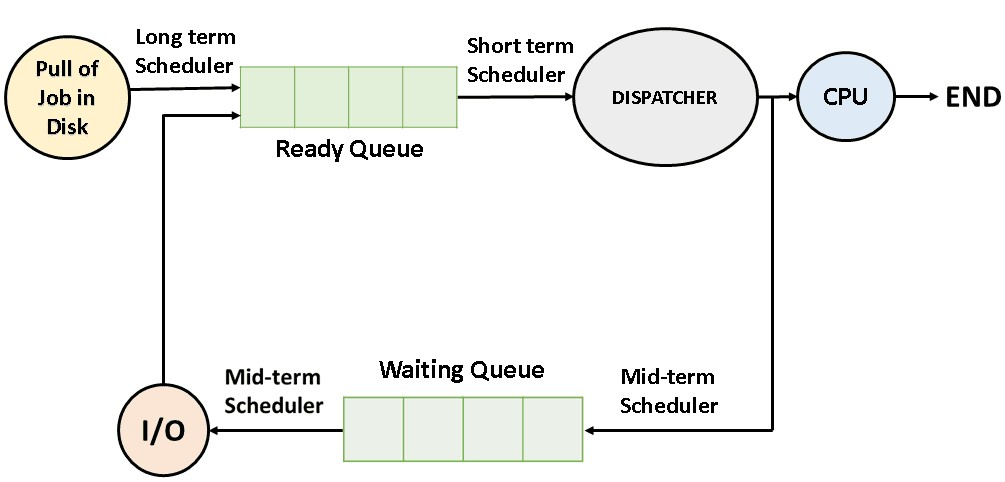
\includegraphics[scale=0.5]{cpu.jpg}
		\caption{Cpu scheduling}
		\end{figure}
		\vskip 1cm

		The project is an attempt to differentiate the behaviour of each scheduler with the statistical approach. In this project we performed each CPU scheduling and compared them on the basis of their completion time,throughput,average job elapsed time and average job waiting time during the process. It also discusses the complexity of the written code as instructed.
		\pagebreak
	  \section*{Software requirement and specification}
		\vskip 1cm
		{\subsection*{Python-dateutil(2.8.1)}
		{The dateutil module provides powerful extensions to the standard datetime module, available in Python.}
		\vskip 1cm
		\subsection*{matplotlib(3.2.2)}
		{Matplotlib is a comprehensive library for creating static, animated, and interactive visualizations in Python.}
		\vskip 1cm
		\subsection*{cycler(0.10.0)}
		{A single entry Cycler object can be used to easily cycle over a single style.}
		\vskip 1cm
		\subsection*{Kiwisolver(1.2.0)}
		{Kiwisolver is an efficient C++ implementation of the Cassowary constraint solving algorithm. Kiwi is an implementation of the algorithm based on the seminal Cassowary paper.}
		\vskip 1cm
		\subsection*{numpy(1.19.0)}
		{NumPy is the fundamental package for scientific computing in Python. It is a Python library that provides a multidimensional array object, various derived objects (such as masked arrays and matrices).}
		\vskip 1cm
		\subsection*{pyparsing(2.4.7)}
		{Pyparsing is a mature, powerful alternative to regular expressions for parsing text into tokens and retrieving or replacing those tokens.}
		\vskip 1cm
		\subsection*{six(1.15.0)}
		{Six provides simple utilities for wrapping over differences between Python 2 and Python 3. It is intended to support codebases that work on both Python 2 and 3 without modification.}
		}
		\vskip 25cm
		\section*{Project Work}
		\vskip 1cm
		{\large{The major aspect of this project work has been to elobrate the main differences that exists between the different aglorithms used in CPU scheduling.\\ The different algorithms and their throghput, average waiting time, average elapsed time etc are plotted using matplotlib and decribed  below using graphs and shapes:-}
		\vskip 2cm
		\subsection*{FCFS}
		{\begin{figure}[H]
		\centering
		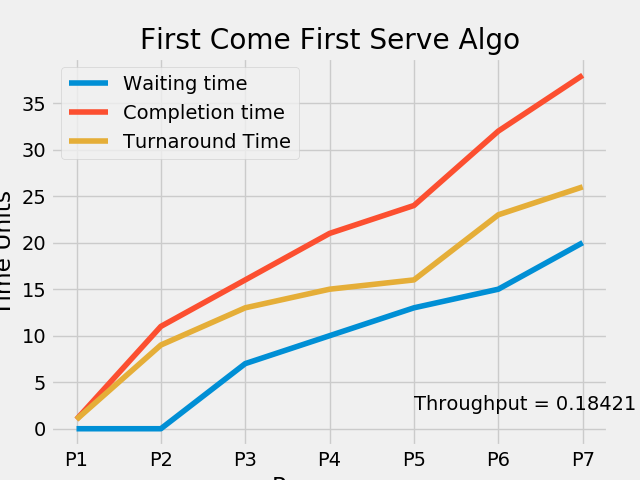
\includegraphics[scale=0.8]{FCFS_output.png}
		\caption{FCFS output values.}
		\end{figure}}
		\subsection*{SJF(Preemptive)}
		{\begin{figure}[H]
		    \centering
		    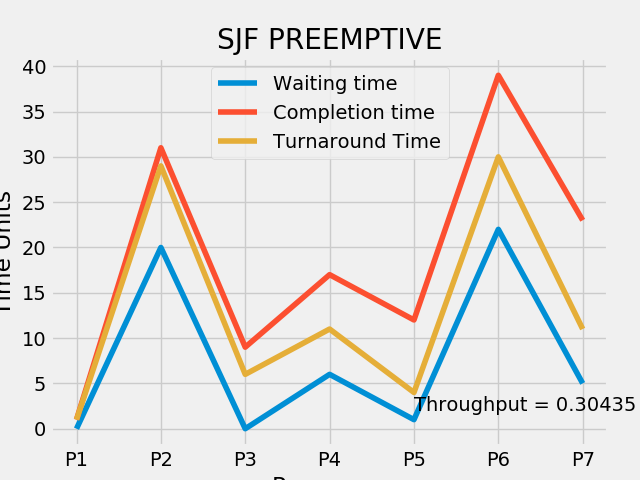
\includegraphics[scale=0.75]{SJF_P_output.png}
		    \caption{SJF(Preemptive) output values.}
		\end{figure}}
		\subsection*{SJF(Non preemptive)}
		{\begin{figure}[H]
		    \centering
		    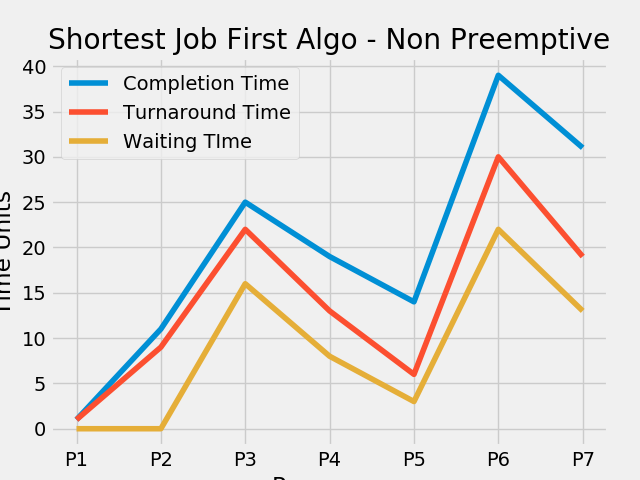
\includegraphics[scale=0.75]{SJF_NP_output.png}
		    \caption{SJF(Non preemptive) output values.}
		    \label{fig:my_label}
		\end{figure}}
		\subsection*{Priorty CPU scheduling(Preemptive)}
		{\begin{figure}[H]
		    \centering
		    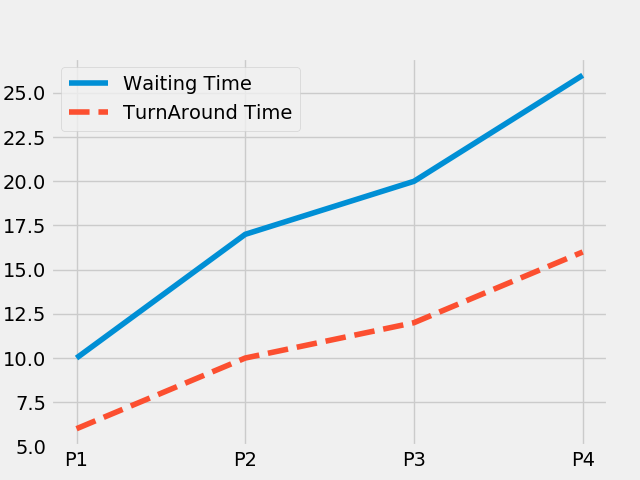
\includegraphics[scale=0.75]{PRIORITY_P_output.png}
		    \caption{Priorty cpu scheduling(Preemptive) output values.}
		\end{figure}}
		\subsection*{Priorty CPU scheduling(Non preemptive)}
		{\begin{figure}[H]
		    \centering
		    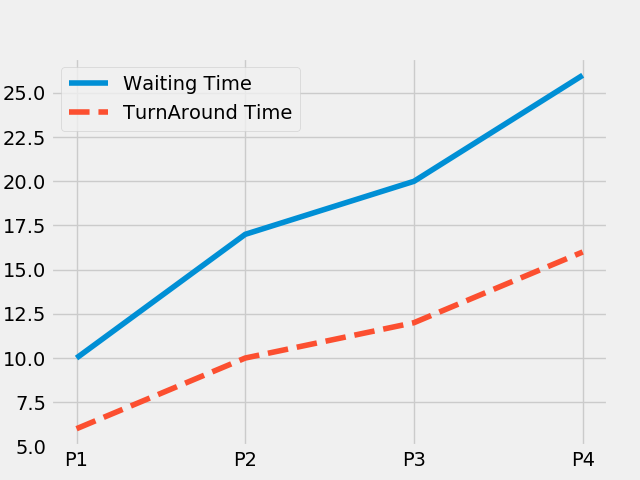
\includegraphics[scale=0.75]{PRIORITY_P_output.png}
		    \caption{Priorty cpu scheduling(Non Preemptive) output values.}
		\end{figure}}
		\subsection*{Round robin CPU scheduling}
		{\begin{figure}[H]
		    \centering
		    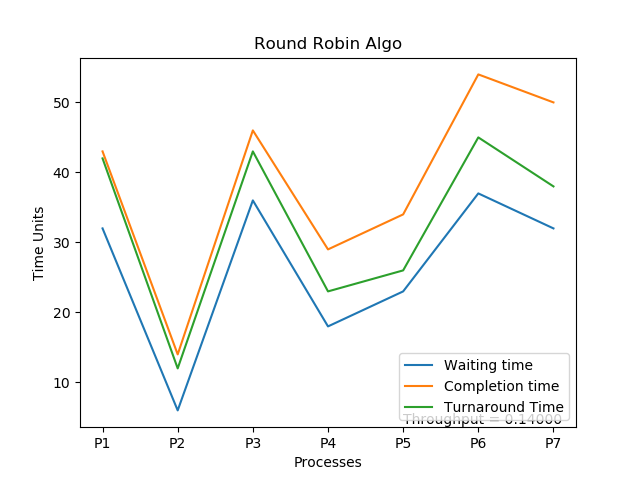
\includegraphics[scale=1]{ROUND_ROBIN_output.png}
		    \caption{Round Robin cpu scheduling output values.}
		\end{figure}}
		}
		\vskip 14cm
		\section*{Conclusion}
		\vskip 1cm
		\large{{From the given project work we have concluded that the difference between the turn around time,average waiting time,average elapsed time and completion time for same input of different cpu scheduling is as follows:-}
		\vskip 1cm
		\begin{figure}[H]
		    \centering
		    \includegraphics[scale=0.9]{compare.png}
		    \caption{comparison between CPU scheduling.}
		\end{figure}
		\vskip 1cm
		\large{from the above graph we came to know that every algorithm works better on the significant problem as the fcfs is better for a small burst time.The sjf is better if the process comes to processor simultaneously and round robin, is better to adjust the average waiting time desired and the priorty works better  where the relative important of each process may be precisely defined.}
		}
		\vskip 15cm

		\section*{References}
		\vskip 1cm
		{\subsection*{}
		{\large{The source code of the project can be found at:-}\\
		  \url{https://github.com/cannibalcheeseburger/cpu-scheduling-simluation.git}\\
	\large{	And the other references we used for this project are given:-}
	\begin{itemize}
	    \item 	A. Dusseau, R. H. dan A. C., Operating Systems: Three Easy Pieces, Arpaci-Dusseau Books, 2014.
	    \item Operating System Principles – Galvin
	    \item Tanenbaum, Modern Operating Systems, Pearson Education, Inc., 2008.
	    \item 	\url{http://www.cs.uic.edu/~jbell/CourseNotes/OperatingSystems/5_CPU_Scheduling.html}
	    \item \url{http://codex.cs.yale.edu/avi/os-book/OS8/os8c/slide-dir/PDF-dir/ch5.pdf}
	\end{itemize}
	}
	}
		
		\end{document}